\section{Zielsetzung}
\label{sec:Zielsetzung}
Ziel des Versuchs ist es die Aufspaltung der Energieniveaus auf Grund des Zeeman-Effektes,
sowie der Hyperfeinstruktur auszumessen. Des Weiteren soll der Landé-Faktor des Gesamtdrehimpulses
des Atoms bestimmt werden. Ebenso soll das transidente Verhalten näher untersucht
werden.

\section{Theorie}
\label{sec:Theorie}

\subsubsection{Magnetisches Moment der Atomhülle}
\label{sec:Atomhülle}

\begin{figure}
  \centering
  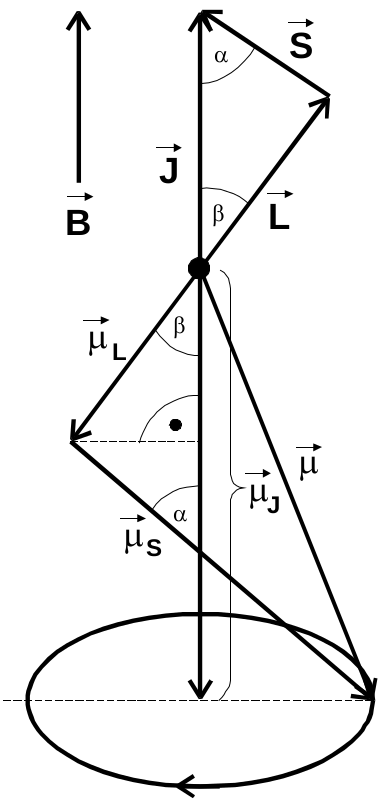
\includegraphics[height=5.5cm]{content/pictures/MagnMoment.png}
  \caption{Skizze zur Veranschaulichung der Zusammenhänge für die Bestimmung des magnetischen Moments der Elektronenhülle.}
  \label{fig:MagnMoment}
\end{figure}

\FloatBarrier
% \begin{figure}
%   \centering
%   \includegraphics[height=5.5cm]{content/pictures/Bild.png}
%   \caption{Bilduterschrift}
%   \label{fig:Bild}
% \end{figure}

% \subsection{Unterkapitel}
% \label{sec:UnterKapitel}

% \begin{equation}
% Für Formeln
%   \label{eqn:Formel}
% \end{equation}
